\chapter{Background}

This chapter...

\section{Software architecture}
The intention of this study is not to contribute to the definition of software architecture, though, our work relies on a shared understanding of what constitutes as the architecture of a system. This section presents the concept of software architecture and the definitions considered in our study.   

During the 1970s,  the idea of organizing software into distinguishable structures was initially introduced. Djikstra \cite{dijkstra_structure_1968} organized the system into a hierarchy of layers, each being dependent upon the interface of the layer below. Parnas discussed the criteria used to modularize systems \cite{broy_criteria_1972}, i.e. responsibility assignment, which allowed for independent development. Further, he introduced the concept of program families \cite{parnas_design_1976} where a set of systems share much of their functionality, allowing for a common design. The work on product families was later extended to describe the process of designing systems that support extensions by using abstracted components \cite{parnas_designing_1979}. 

However, the term \textit{software architecture} was formally introduced by Perry and Wolf in \cite{perry_foundations_1992}, where they defined software architecture as:

\[ Software \;  Architecture = \{elements,form,rationale\} \]

In words, software architecture is defined as a set of architectural elements that persist in a particular form. Form relates to the properties of each element and the relationship between elements. To make an architecture explicit, Perry and Wolf \cite{perry_foundations_1992} suggest the usage of views to represent different aspects of the architecture. 

Related to that of a specific architecture, Perry and Wolf \cite{perry_foundations_1992} define an architectural style as a generalization of various similar architectures. Garlan and Shaw \cite{ambriola_introduction_1993} extended the knowledge by providing a list of architectural styles that were commonly used in the design of software systems, these include \textit{pipes and filters}, and \textit{layered systems}. Perhaps more importantly, Garlan and Shaw \cite{ambriola_introduction_1993} describe the rationale of using a specific style and the trade-offs between styles.

Today, there are mainly two definitions of software architecture:

\begin{itemize}
    \item \textbf{Bass et Al \cite{bass_software_2013}}: \say{The software architecture of a program or computing system is the structure or structures of the system, which comprise software elements, the externally visible properties of those elements, and the relationships among them.}
    \item \textbf{Jansen and Bosch \cite{jansen_software_2005}}: \say{The composition of a set of architectural design decisions} where a design decision represents \say{A description of the set of architectural additions, subtractions and modifications to the software architecture, the rationale, and the design rules, design constraints and additional requirements that (partially) realize one or more requirements on a given architecture.}
\end{itemize}

While both definitions acknowledge that a system should always meet the functional requirements and that the process of creating the architecture is a balance between quality attributes, it is the former definitions that lend itself naturally to structural analysis.

Finally, in many references to architecture, the term design is often used ambiguously. To remedy this, Eden and Kazman \cite{eden_architecture_2003} formalized the hypothesis of an intension and locality criteria. A specification is said to be intensional if there are infinitely many ways of realization, all others are extensional. Further, a specification is said to be local if it only affects a small part of a program. Architectural specifications are both intensional and non-local, whereas design level specifications are intensional and local.

\section{Architectural security constraints}

The purpose of software and architectural security is to ensure that no harm occurs to the systems assets in the presence of malicious actors \cite{mcgraw_software_2004}. Assets are identified by the needs of the systems stakeholders and may be tangible (e.g, cash) or intangible (e.g, information) \cite{haley_security_2008}. At the core of software security are the following four concerns, often refereed to as CIAA:

\begin{itemize}
    \item \textbf{Confidentiality}, \say{Preserving authorized restrictions on information access and disclosure.} \cite{ross_systems_2018}
    \item \textbf{Integrity}, \say{Guarding against improper information modification or destruction.} \cite{ross_systems_2018}
    \item \textbf{Availability}, \say{Ensuring timely and reliable access to and use of information.} \cite{ross_systems_2018}
    \item \textbf{Accountability}, \say{Ensuring that it is possible to trace security relevant actions (i.e., subject-object interactions) to the entity on whose behalf the action is being taken} \cite{ross_systems_2018}
\end{itemize}

These concerns relate to a system's security goals as a violation of a concern to one of the assets describe a possible threat \cite{haley_security_2008}. Security requirements later operationalize the security goals and constrain the architecture of a system. As security is often considered a quality attribute, the satisfaction of a security requirement becomes a risk management issue.  Highly valuable assets should warrant a higher degree of protection and consequently, require stronger constraints on the architecture \cite{broy_software_2007}.

While the term architectural constraint means anything that limits the set of design choices, several concepts have come to form a generalizable knowledge at different levels of abstraction. 

\textbf{Security principles}, such as those proposed by OWASP\footnote{\url{https://blog.threatpress.com/security-design-principles-owasp/}}, are defined at a level of high abstraction that allows them to be used on almost any component in a system. Examples of such principles include \textit{The principle of least privilege}, stating that any user should have the least amount of privileges needed to perform an action. While the abstraction of principles enables them to apply to most components of a system, it also means that an architect has to assess, instead of precisely knowing, whether a designed conforms to the principle. 

\textbf{Security patterns} are at a lower level of abstraction as they represent "encapsulated solutions to recurrent system problems" \cite{fernandez-buglioni_security_2013}. By providing a generalizable solution to a known problem, patterns help to bridge the gap between the developers and the architectural experts \cite{rosado_study_2006}. The extensive knowledge of security patterns and their implementation also allows for comparison in terms of their impact on other quality attributes, such as maintainability and performance \cite{scandariato_architecting_2009}. 

\textbf{Security rules}

\section{Static analysis}\todo{static analysis}
\cite{chess_secure_2007}

\cite{pistoia_survey_2007}

Information flow analysis \cite{hutchison_information_2005} from which we lend ideas for our extension


\subsection{ArchUnit}\label{archunit-back-section}
ArchUnit is a library that leverages static analysis of Java bytecode to validate architectural constraints. These constraints are expressed in Java code and can be validated using conventional unit testing frameworks, which enables the constraints to be validated in a continuous integration setting.

In ArchUnit, architectural rules are expressed against a representation of the analyzed system. This representation is composed of the constructs outlined in Figure~\ref{fig:archunit}. Most notably:

\begin{itemize}
    \item Methods, constructors and static initializers, i.e. anything that contains code statements, are collectively referred to as \textbf{code units}.
    \item Fields and code units, i.e. constructs that are owned by a class, are known as \textbf{members} of that class.
    \item Field accesses, method calls and constructor calls are collectively known as \textbf{accesses}. An access has a source, i.e. the code unit from which the access originates, and a target, i.e. the member that is being accessed.
\end{itemize}

\begin{figure}
    \centering
    \captionsetup{justification=centering}
    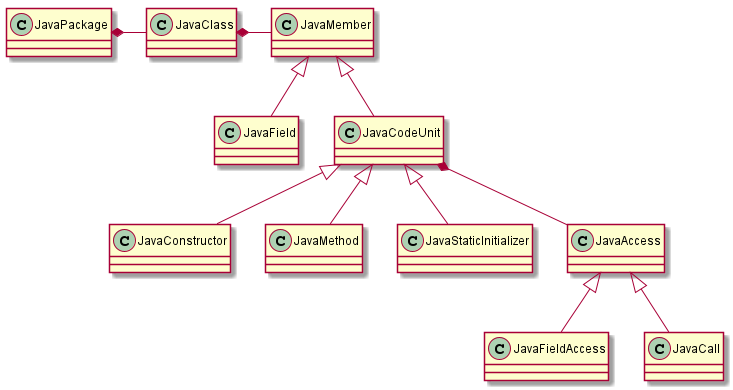
\includegraphics[width=\textwidth]{figure/ArchUnit.png}
    \caption{The architectural constructs present in the domain of ArchUnit, adapted from [...].}
    \label{fig:archunit}
\end{figure}

\section{Related Work}\todo{related work}

\subsection{Architectural conformance monitoring}
\cite{aldrich_archjava_2002}, \cite{abi-antoun_analyzing_2010}, \cite{luckham_event-based_1995}, \cite{abi-antoun_static_2009}, \cite{de_silva_controlling_2012}, \cite{knodel_comparison_2007} 



\subsection{Security annotations and Architectural description languages}
\cite{sabo_preserving_2009}



